
%%%%%%%%%%%%%%%%%%%%%%%%%%%%%%%%%%%%%%%%%%%%%%%%%%%%%%%%%%%%%%%%%%%%%%%%%%%%%%%%

%        1         2         3         4         5         6         7         8

\documentclass[letterpaper, 10 pt, conference]{ieeeconf}  % Comment this line out if you need a4paper

%\documentclass[a4paper, 10pt, conference]{ieeeconf}      % Use this line for a4 paper

\IEEEoverridecommandlockouts                              % This command is only needed if 
                                                          % you want to use the \thanks command

\overrideIEEEmargins                                      % Needed to meet printer requirements.


\usepackage{graphics} % for pdf, bitmapped graphics files
\usepackage{epsfig} % for postscript graphics files
\usepackage{mathptmx} % assumes new font selection scheme installed
\usepackage{times} % assumes new font selection scheme installed
\usepackage{amsmath} % assumes amsmath package installed
\usepackage{amssymb}  % assumes amsmath package installed

\usepackage[font=small,labelfont=bf]{caption}

% Other package
\usepackage{tikz}
\usepackage{graphicx}
\usepackage{caption} 
\usepackage{subcaption}
\usepackage{multirow}
\usepackage{array}
\usepackage{booktabs}
\usepackage{hyperref}

\usepackage{pdfpages}
\usepackage{caption}
%\usepackage{geometry}
\usepackage{import}
\usepackage{standalone}

\title{\LARGE \bf
  Team-JSK: MBZIRC Progress Report 2
}
\author{\textbf{Team JSK} ({\texttt{www.jsk.t.u-tokyo.ac.jp}})% <-this % stops a space
  \\ JSK Lab, Graduate School of Information Science and Technology,
  The University of Tokyo \\
  7-3-1 Hongo, Bunkyo-ku, Tokyo, Japan 113-8656.  \\
}

\begin{document}

\maketitle
\thispagestyle{empty}
\pagestyle{empty}


\section{INTRODUCTION}
This document provides the second report of 
Team JSK's progress in preparing
for the Mohamed Bin Zayed International Robotics Challenge
(MBZIRC). The document highlights some of the advances made since the submission of the first progress report as well as future plans leading to the actual challenge. 


\section{PROJECT PERSONNEL}
Team JSK is currently made up of 13 members: Prof. Masayuki Inaba, Prof. Kei
Okada, Dr. Yohei Kakiuchi, Dr. Wesley Chan, Bakui Chou, Xiangyu Chen,
Krishneel Chaudhary, Kohei Kimura, Yuki Furuta, Hiroto
Mizohana, Fan Shi and Tomoki Anzai. The team is roughly divided into
three groups corresponding to each task with groups having overlapping
personnel.

\section{CHALLENGE 1: LANDING UAV ON A MOVING VEHICLE}

%Copyright (C) 2016 by Krishneel@JSK Lab, The University of Tokyo

%Copyright (C) 2016 by Krishneel@JSK Lab, The University of Tokyo

\documentclass{standalone}
\usepackage{footnote}
\usepackage{hyperref}
\usepackage{graphicx}
\usepackage{fancyhdr}

\renewcommand\footnoterule{%
  \kern-3\p@
  \hrule\@width2.5cm
  \kern2.6\p@
}
\makeatother

\begin{document}

\section{Software}


\subsection{Software Environment}
The motion planning and visual perception algorithms are implemented
on Robot Operating System (ROS) environment\footnote{\url{http://www.ros.org}}.
We used Gazebo\footnote{\url{gazebosim.org}} for virtual simulations
\footnote{\url{https://github.com/start-jsk/jsk_mbzirc}}. Our
algorithms are implemented in C/C++, Python and CUDA-C.


\subsection{Visual Perception}

The image processing is one of the fundamental component of autonomous
systems. With efficient and robust image processing the planning and
decision making can be done more readily which improves the accuracy
and robustness of executing the assigned task. Hence, one of our
primary objective while designing our software architectures was
real-time performance with minimal loss of accuracy. The visual
components of task one include three main stages described as follows:

\subsubsection{Target Detection}
The target detection phase is the initial localization of the landing
region (heliport) on the truck. To detect the heliport we use the
traditional computer vision detection approach where by a sliding
window based method is used. However such raster scanning windows are
computationally expensive even for high end systems. To overcome this
crucial limitation we first generate candidate objectness
regions. Since the heliport is fixed to a moving target, we use
Gaussian based background subtractor fused with Kalman Filters for 
global motion compensation to generate regions of interest
(ROI)  with stable changes. The candidate ROI's are then ranked using
edge similarity between each sliding window. High scoring ROI are then
used for detecting the heliport using pretrained detector. 
Let $\mathbf{H}$ denote the detected target region.

\subsubsection{Target Tracking}

In order for an UAV to approach and land on the heliport online visual
feedback is very important given that the target is constantly moving.
Using the assumption that the target is not
expected to change abruptly both in terms of visual motion and
appearances, we use visual tracking for online feedback.
The detected region $\mathbf{H}$ is used to initialize the
tracker. Our visual tracking algorithm is highly efficient and robust
to both scale and visual changes and runs in real time, thus
providing frame by frame location of the target. To enable a tracker
to run online in real time we carefully crafted the expensive process
of feature computation by reducing it to one time process. 
The invariant features for tracking are computed by passing the image
through several pre-trained kernels of varying dimensions. By varying
the sizes of the kernel, an approximate scale can also be detected.
Moreover, the tracker is updated online at fixed intervals.

\begin{figure}[t!]
  \centering
  \includegraphics[height=1in]{sections/task1/images/detect2}
  \includegraphics[height=1in]{sections/task1/images/detect1}
  \caption{Illustration of truck and heliport detection.}
\end{figure}

\subsection{Results Achieved to Date}

We have completed task one fully autonomously landing on the moving
target at 5km/h, 10km/h and 15km/h. The results of these landings are
shown in video. Moreover we demonstrate the effectiveness of our real
time planning and tracking by showing the results of long time
following of the target at over 35km/h. 

\end{document}


%% insert yout latex module file here. the contents should go to the
%% tasks folder under section


\section{CHALLENGE 2: OPERATING A VALVE STEM}

%Copyright (C) 2016 by Krishneel@JSK Lab, The University of Tokyo

\documentclass{standalone}
\begin{document}

\section{example}

This example.tex shows how to write the module


\end{document}

\section{CHALLENGE 3: SEARCH, PICK AND PLACE}

%Copyright (C) 2016 by Krishneel@JSK Lab, The University of Tokyo

\documentclass{standalone}
\begin{document}

\subsection{Platforms}
For task 3, we used customized DJI M100 as our platform which had been introduced in task 1. We equipped Nvidia Jetson TX1 and TK1 based embedded computer to do both control and vision algorithms. The magnets gripper is redesigned to be stronger to pick the objects and also for the drone to fly more stable. Temporarily we did the real world test through remote operation, we are also trying to set up the network configurations which is given by the MBZIRC committee recently. Also we accelerate our vision algorithm in gazebo simulation as we showed in the first report. For now we are trying to develop a semi-autonomous approach for task 3 considering the difficulties we meet in manually operation.

\subsection{Magnet Gripper Design}
The reason we choose electronic magnet is that it is easy to control if we design the circuits ourselves. The ordinary seems stronger but it may requires executor unit to push the object down when the drone will to release the object, which will make the attachment more complex and additional motor is needed. We also considered to use a air vacuum like our team in Amazon Picking Challenge, but the size of vacuum is too big for the drone in our case. 

We equipped 5 small electronic magnets for a gripper of size $10cm \times 10cm$. Each electronic magnet is capable of more than $20N$ holding force if the objects are thick enough. However, according to our experiment, since each object is less than $500g$, the thickness will be less than $1.6mm$ if the object is a square of $20cm \times 20cm$ and made of pure iron(Consider the density of iron to be $7.86g/cm$). In addition, if the surface of the object is too big, the propeller effect will happen and therefore request the electronic magnets to be more powerful. Temporary our gripper with $5$ electronic magnets can pick the object of almost $1kg$ of the thickness of the iron is more than $0.3mm$. 

Five touch sensors are equipped on the gripper with the electronic magnets to detect the contacts between the object and the gripper. Besides, five touch sensors will bring the position information of the gripper compared to the object since sometimes only $2$ or $3$ touch sensors are triggered and then we know the offset of the gripper and the object. 

The design of the electronic magnet circuits driver is simple since it can be simply regarded as a series connection of a inductor and a small resistor, Darlington Transistor will be enough to driver a electronic magnet since the current request is only $200ma$. Because of the inductor effect, a protection diode is very necessary in the circuits. We designed the circuits board with a $32$ bits micro controller, a Darlington driver IC and both serial, CAN communication interface in the gripper board. We write a ROS node in the board and it can directly report the status of the magnets and touch sensors in the gripper and also receive the orders from the embedded computers. 

\subsection{Teleoperation for Task 3}
At this moment, we only perform the real platform experiment through teleoperation by human beings. When we control the UAV manually to pick the object, we figure out it is not a easy job for real UAV platform compared to the simulation since it is very difficult to control the UAV accurately to approach the object, in addition, the ground effect will unstable the UAV when the UAV is getting close to the ground. We address this problem by hanging the magnet gripper with a spring so that the UAV can pick the object without getting too close to the ground. However this may introduce another problem that the gripper will be shaking whenever the uav change the velocity, we are also addressing this problem now and try to get a stronger hanging method to make the gripper relatively stable.

We tested on only one UAV and it seems we can picking $5$ static objects within $8$ minutes, the time could be improved if we adopt the semi-autonomous teleoperation method like store the global position of the box to drop the objects and after pick the object, the UAV can directly move to the global position of the aim box.


\end{document}


\section{GRAND CHALLENGE}

%Copyright (C) 2016 by Krishneel@JSK Lab, The University of Tokyo

\documentclass{standalone}

\usepackage{graphicx}
\usepackage{float}
\floatstyle{boxed} 
\restylefloat{figure}

\begin{document}

\subsection{Setup of TestBed}

We have prepared our testbed where we will perform the outdoor testing in the real world is located in Hachioji, Tokyo, Japan as shown in Fig.\ref{fig:objects}. As far we developped the robot system for each task in this testbed individually. 

 \subsection{Future Work}
 Once we complete each of the three tasks above, for the grand challenge we will combine each of the 3 tasks above, however we plan to make some changes such as UAV to UAV and UAV to UGV communications such that all the robots are able to collaborate in completing the tasks.
 
\begin{figure}[h]
   \newcommand \ilenght{0.1}
   \newcommand \iheight{2.0in}
   \newcommand \iwidth{0.46\textwidth}
   \centering
   \subcaptionbox{
     \scriptsize{}\label{fig3:a}}{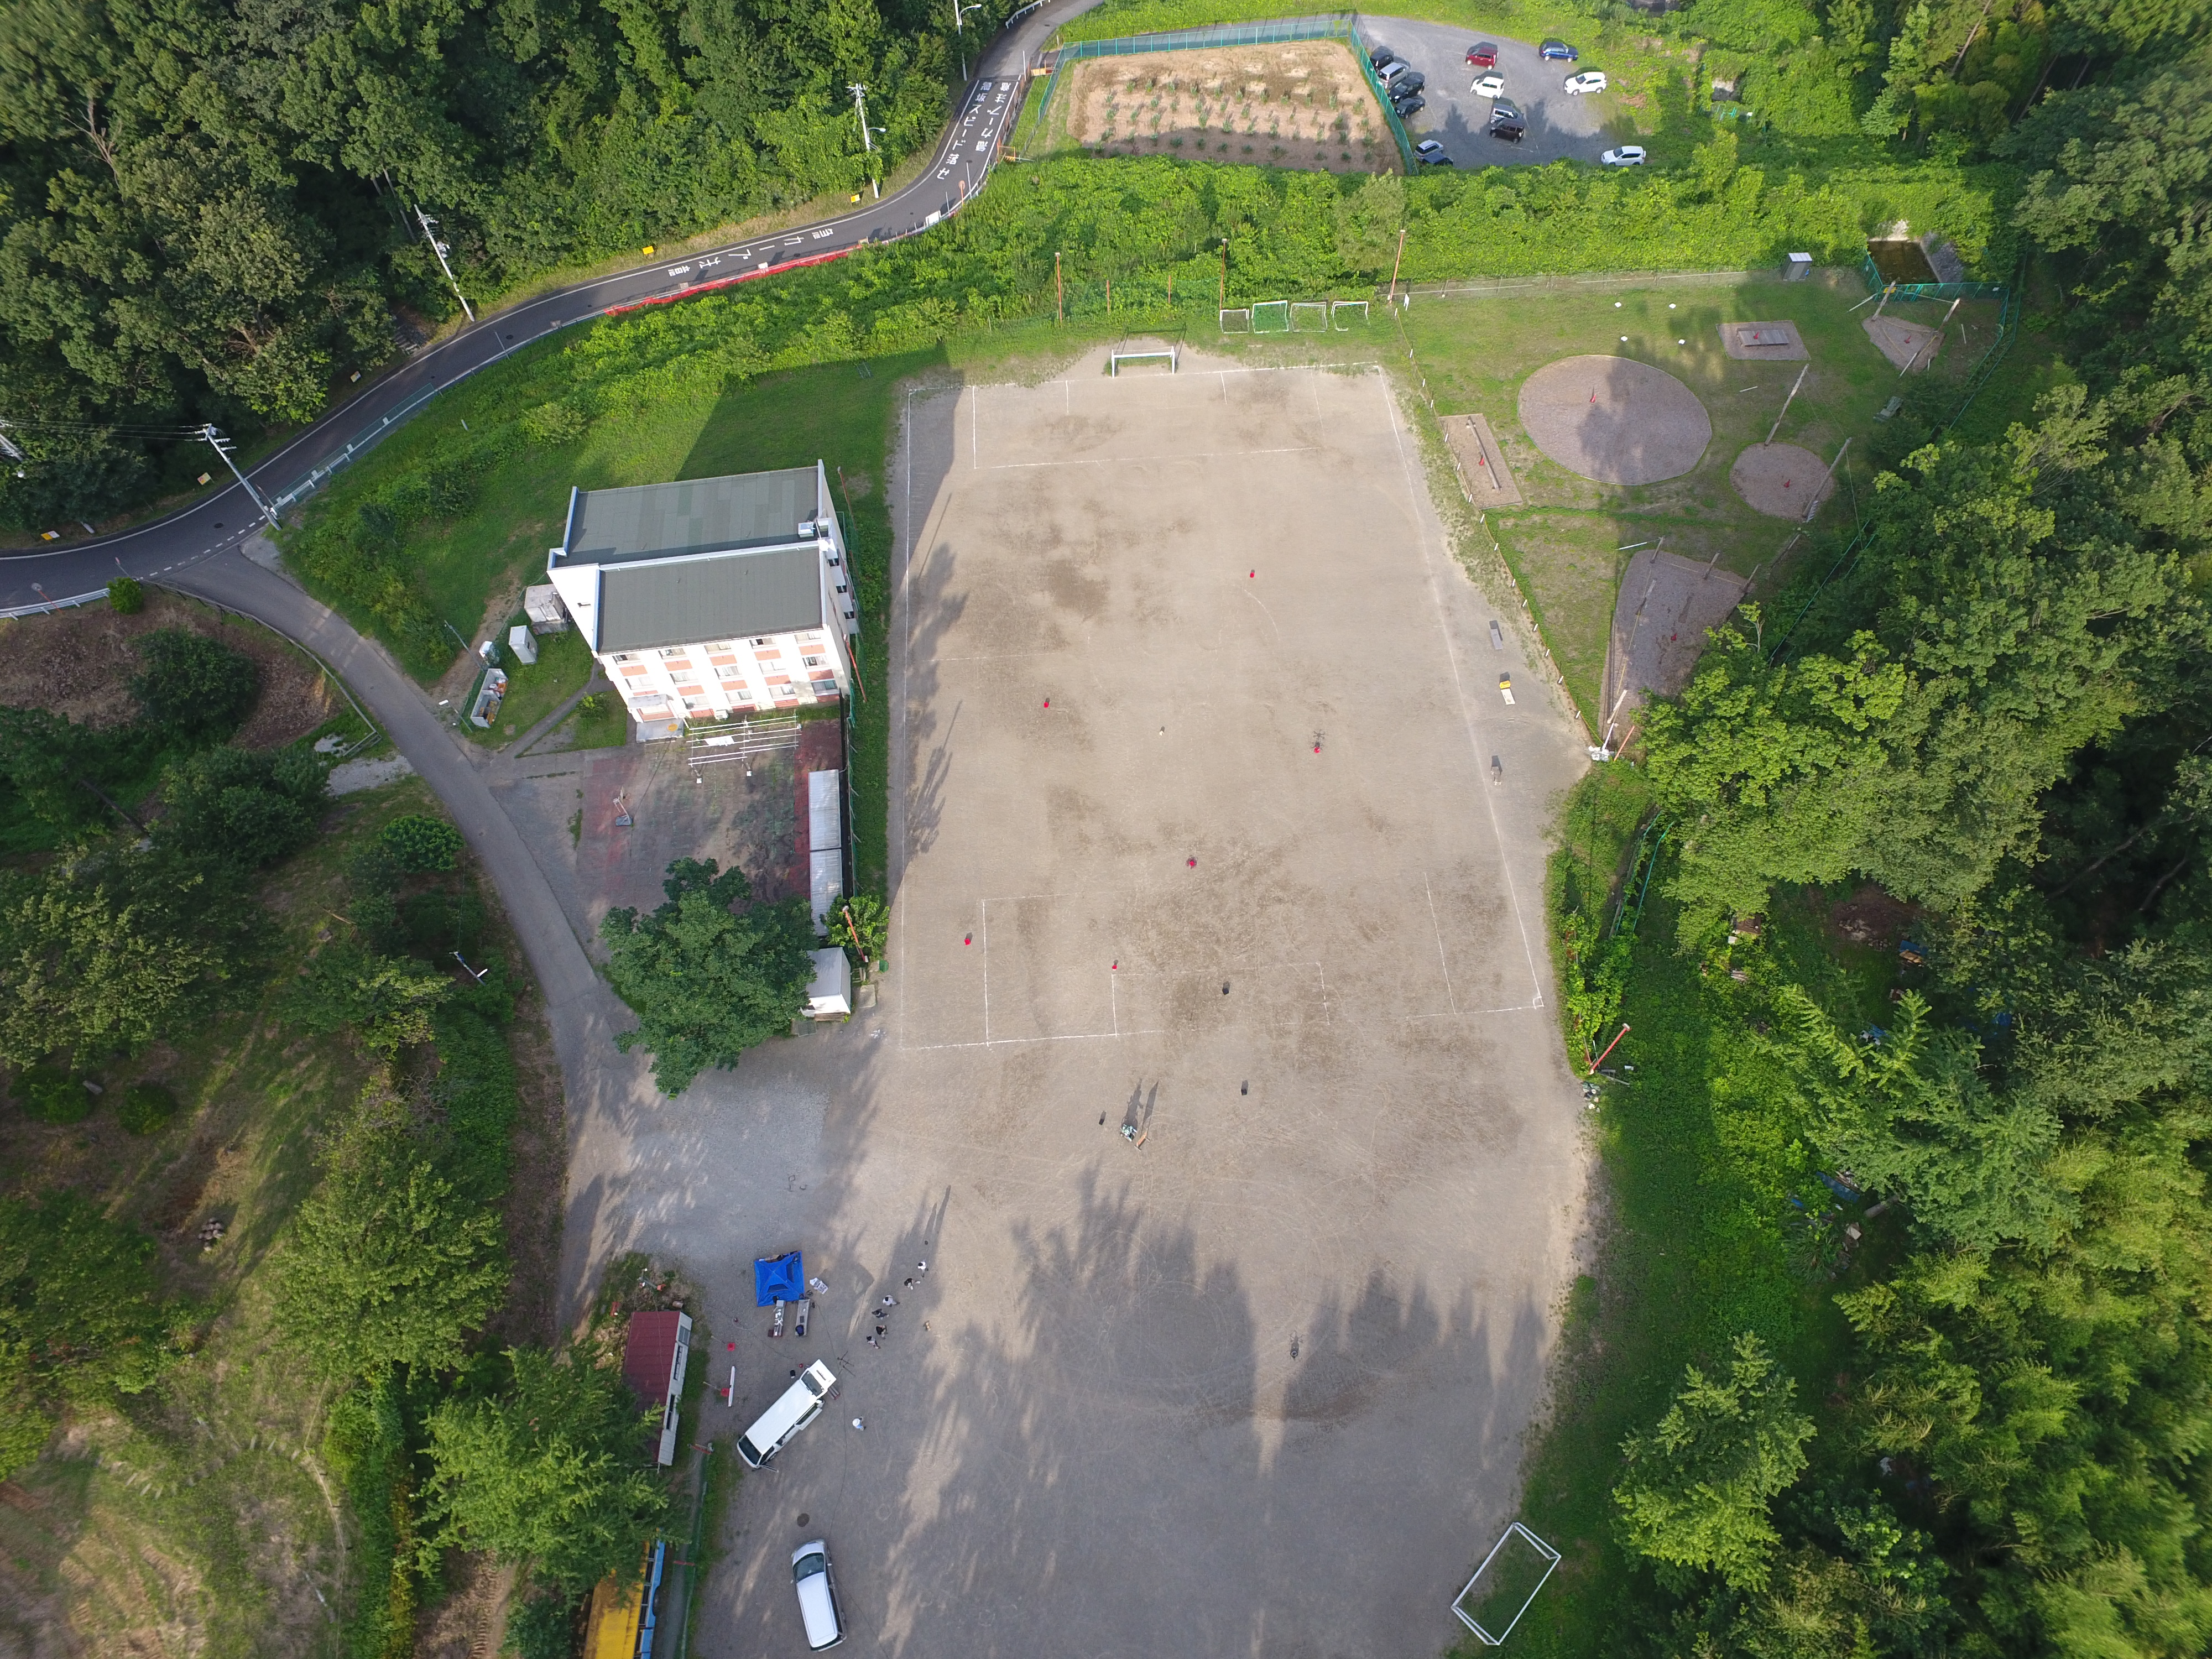
\includegraphics[width=\iwidth, height=\iheight]{sections/grand/images/DJI_0028}}\hspace{1.1em}%
   \subcaptionbox{
     \scriptsize{}\label{fig3:b}}{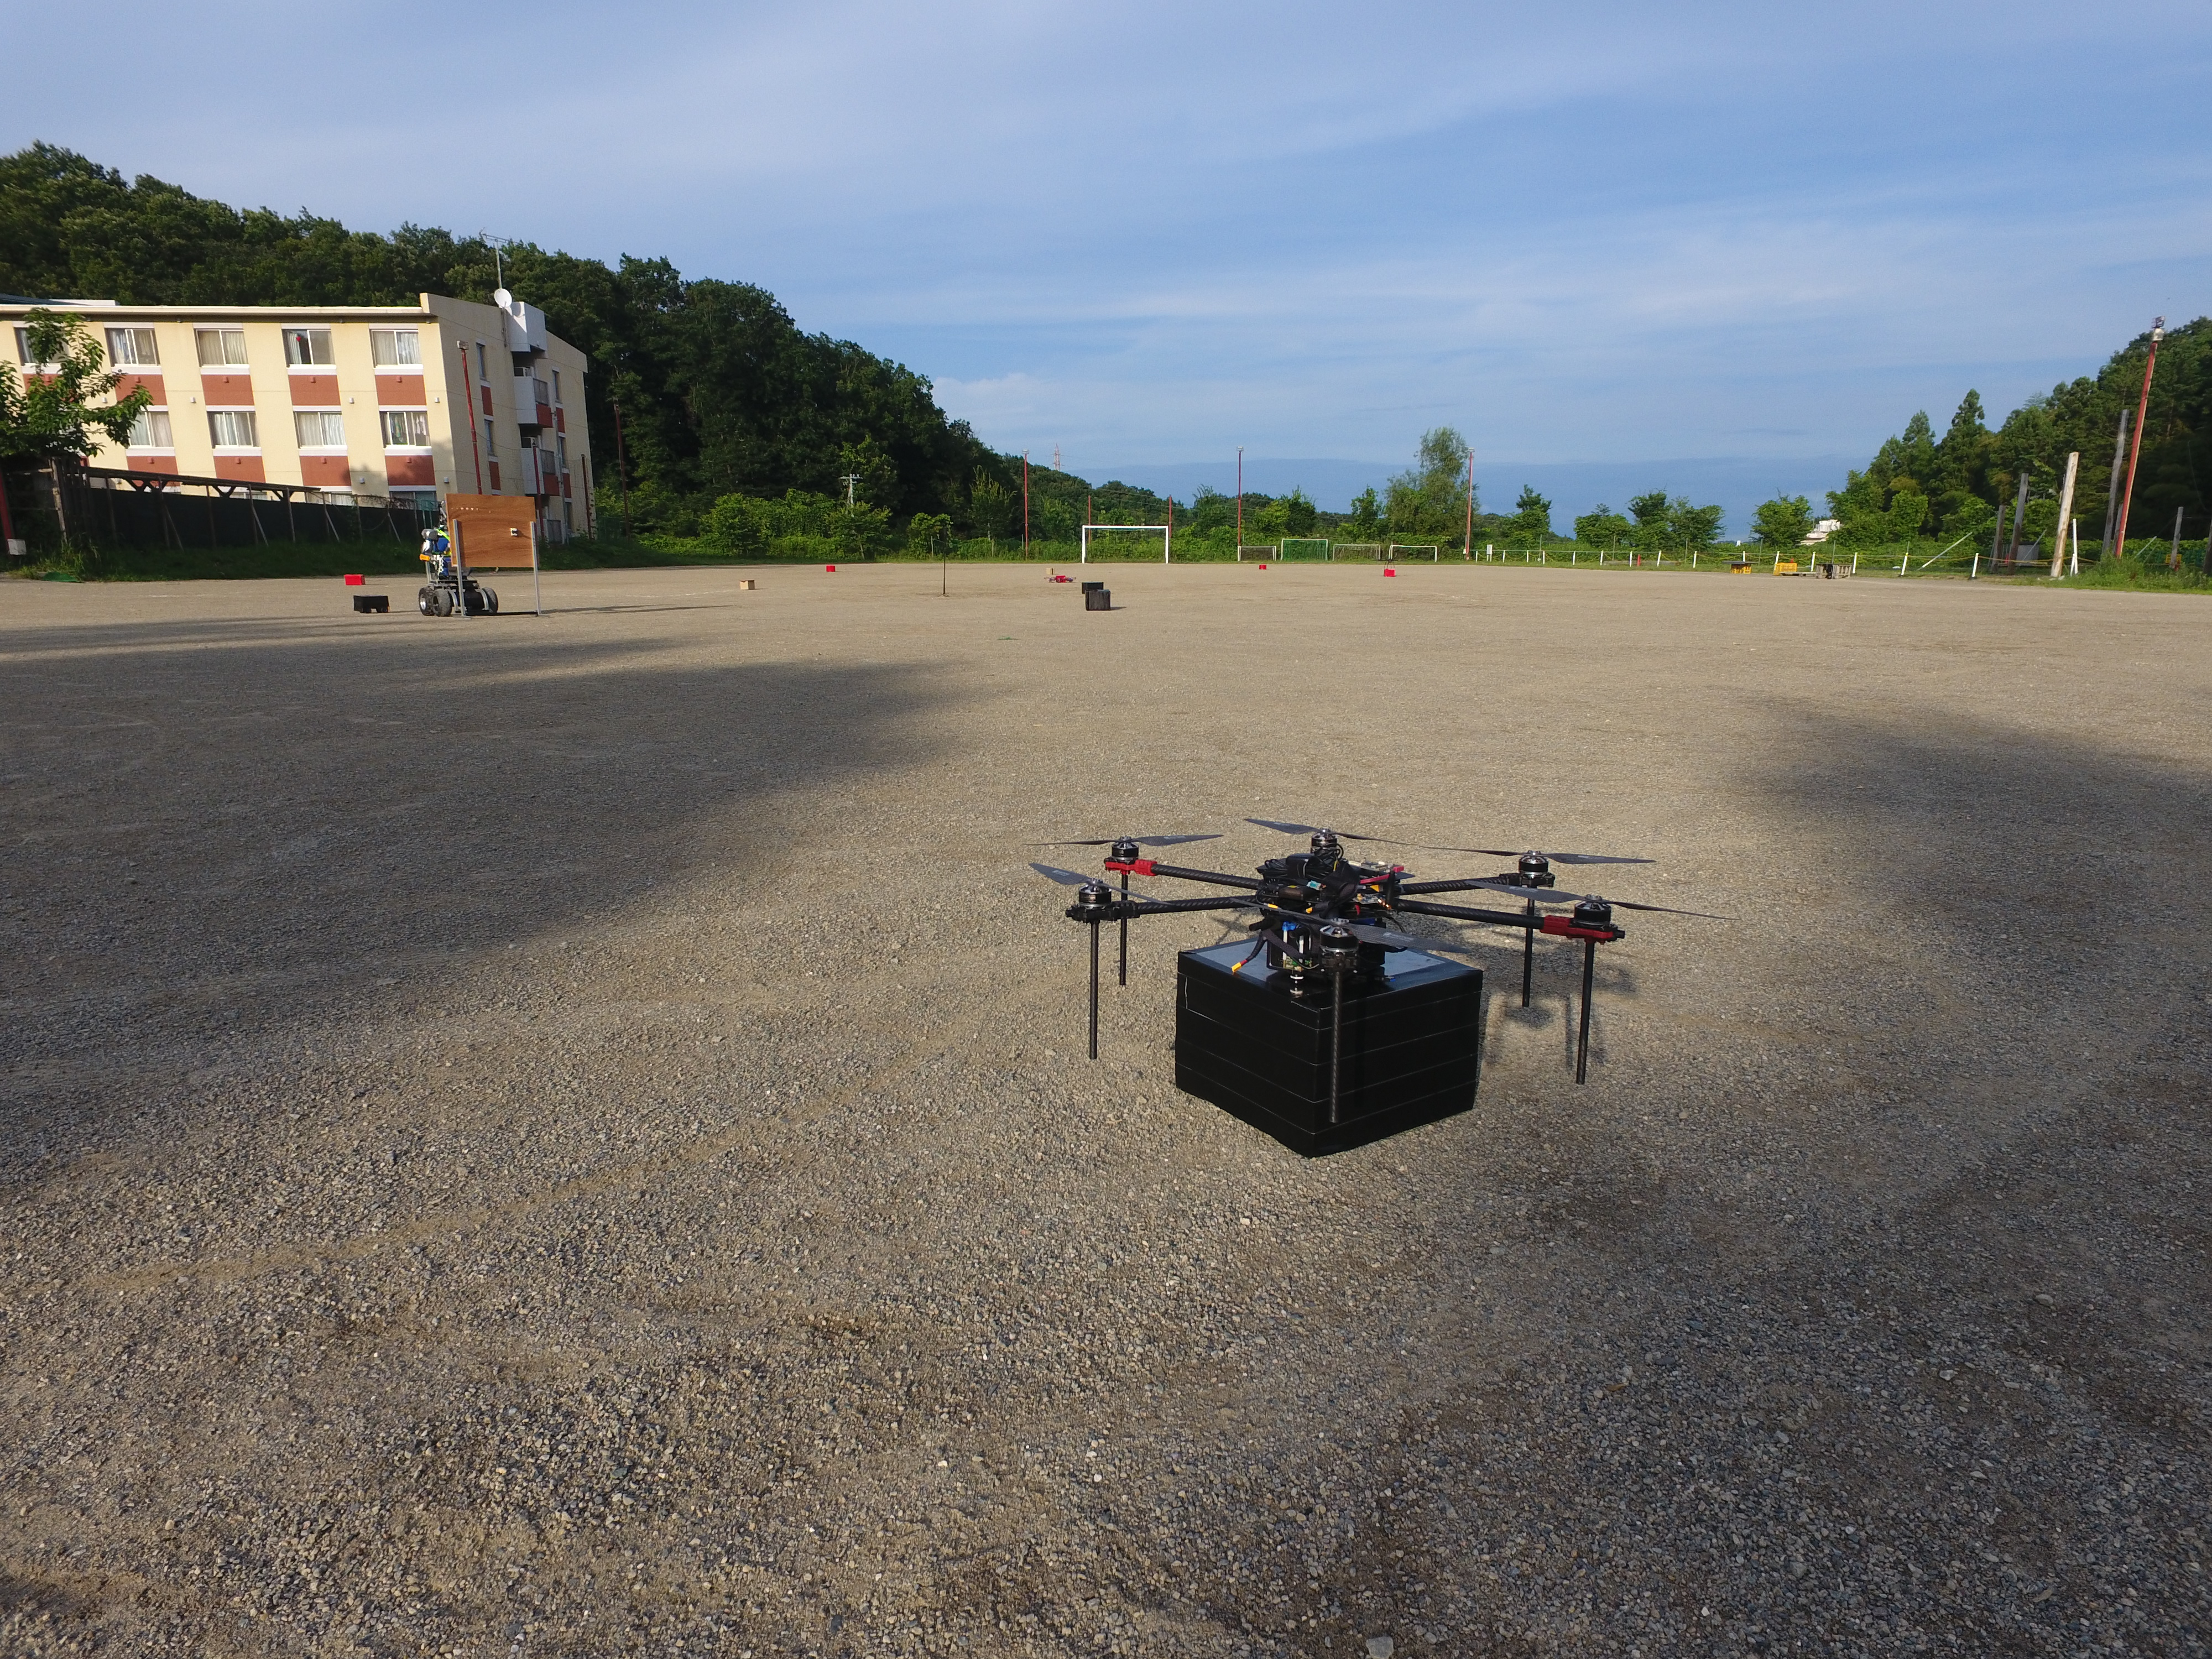
\includegraphics[width=\iwidth, height=\iheight]{sections/grand/images/DJI_0059}}\hspace{1.1em}%
   \subcaptionbox{
     \scriptsize{}\label{fig3:c}}{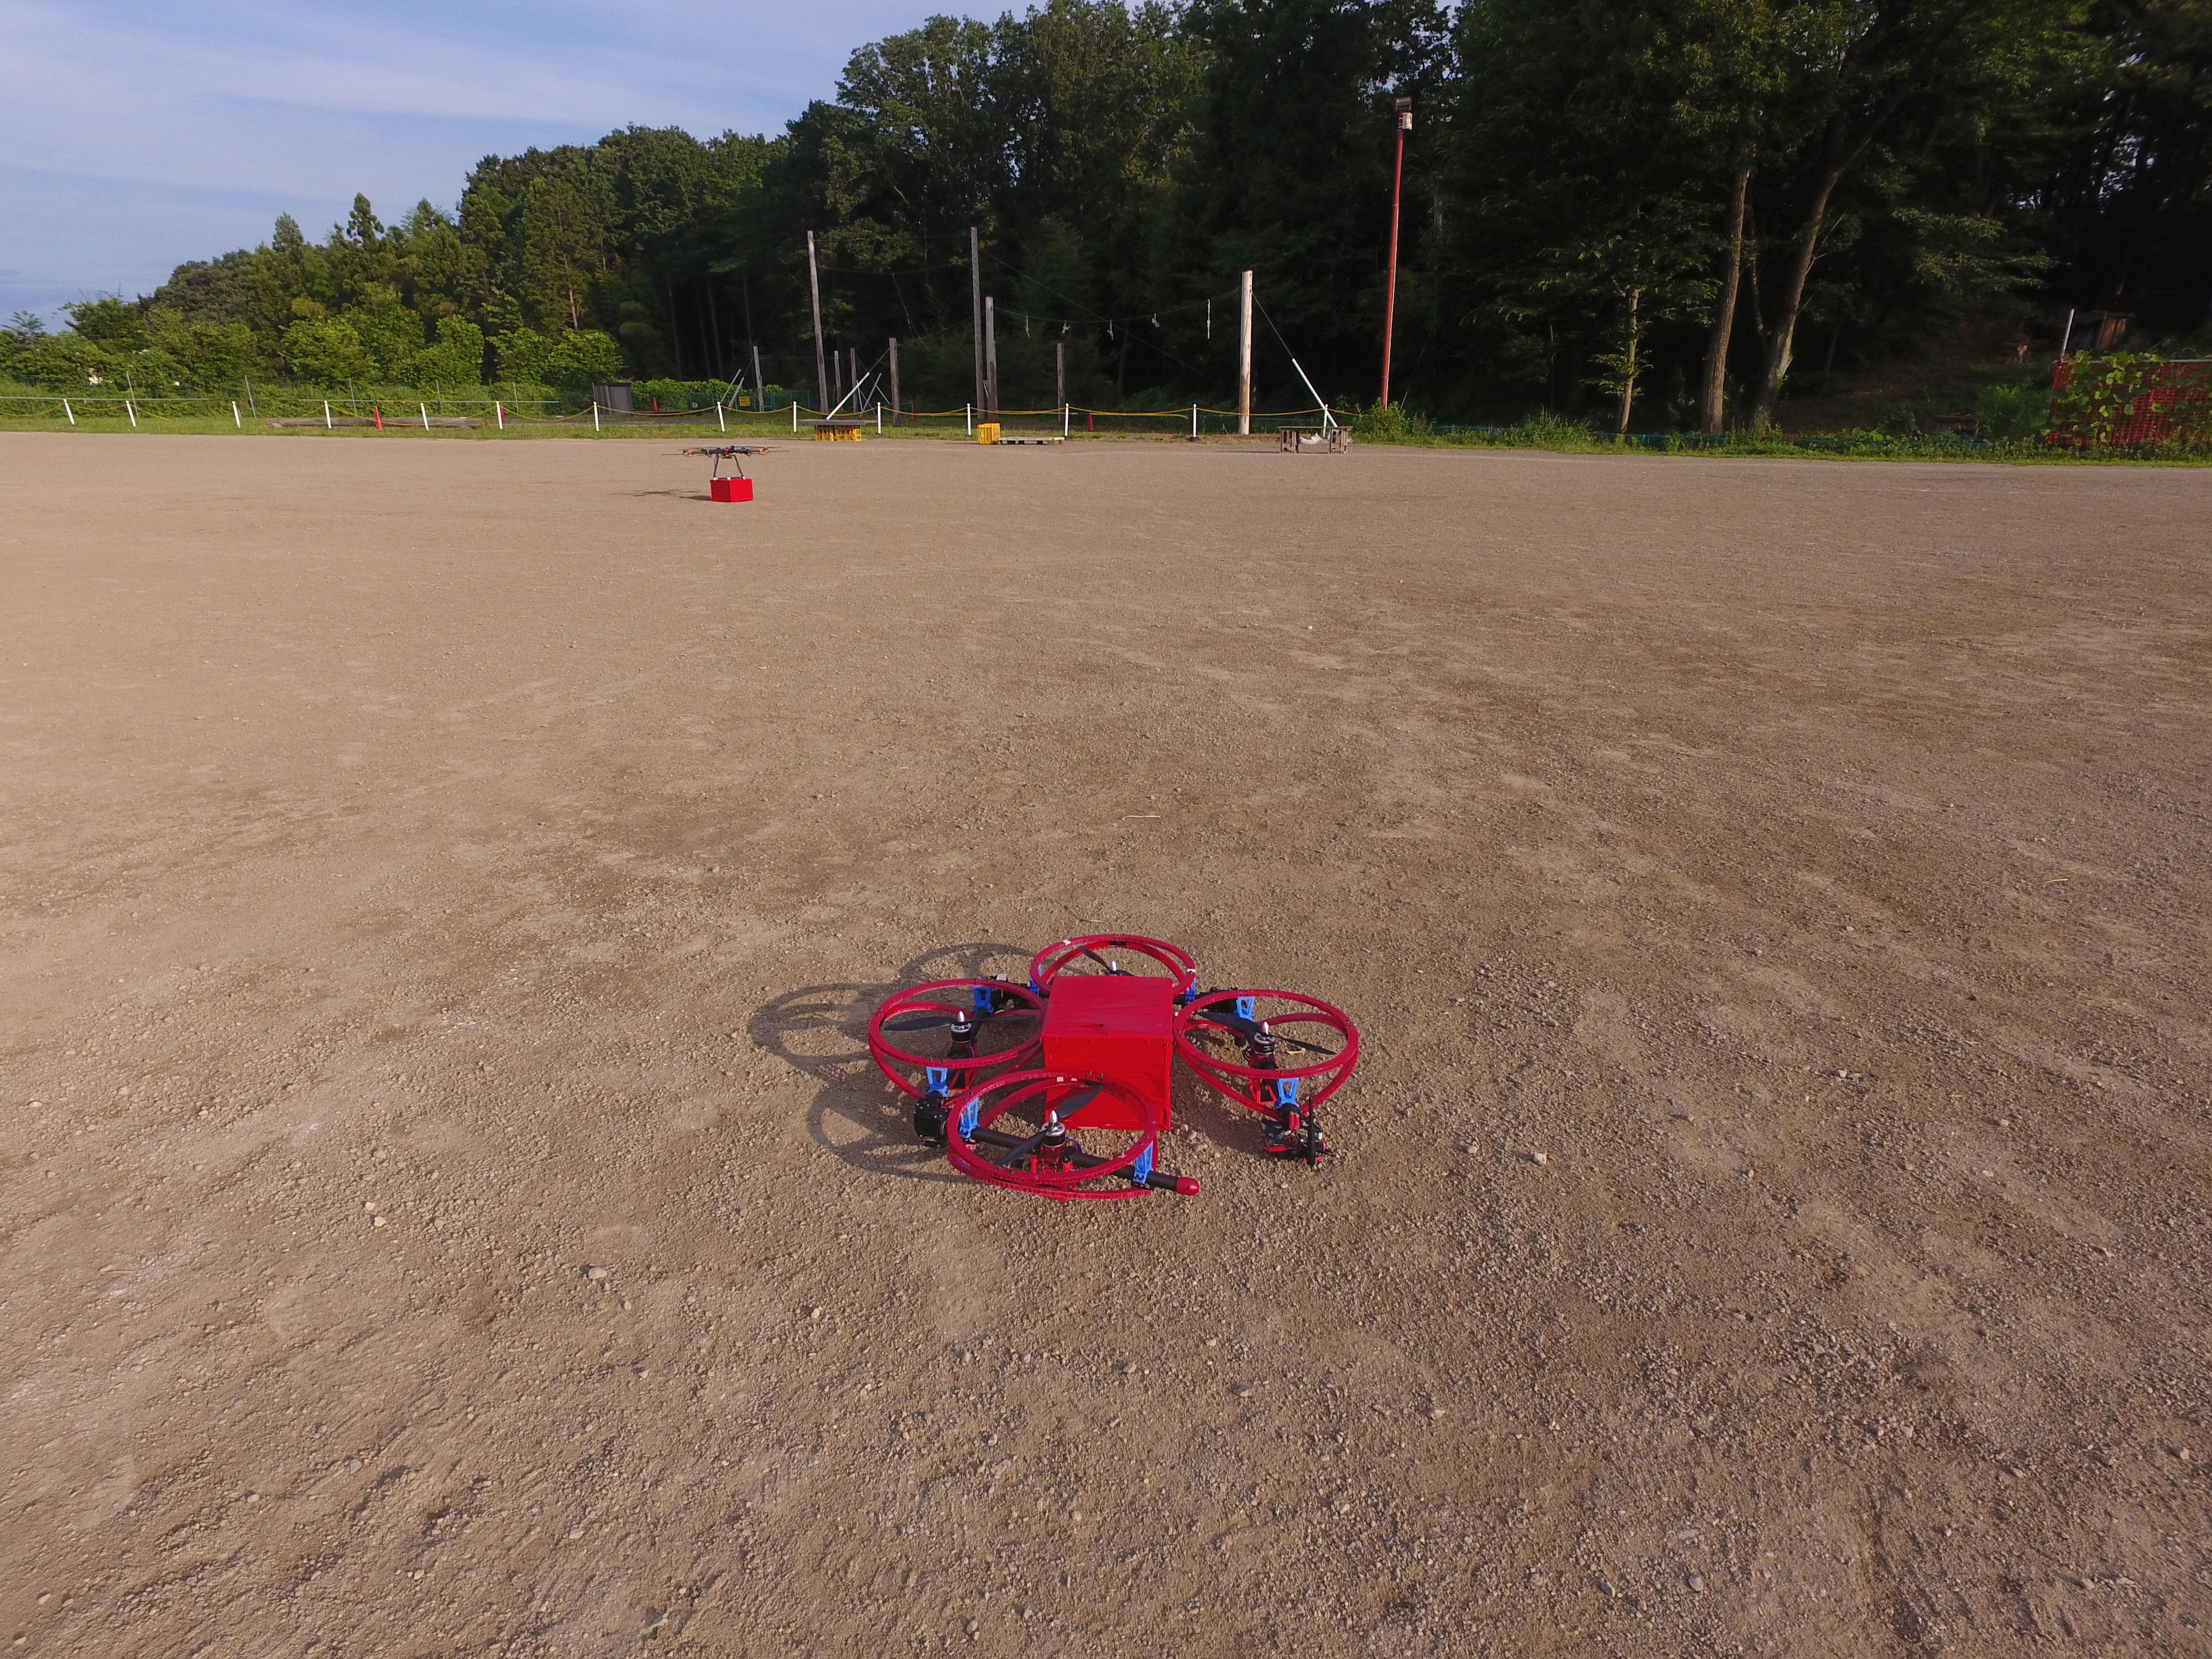
\includegraphics[width=\iwidth, height=\iheight]{sections/grand/images/DJI_0079}}\hspace{1.1em}%
   \subcaptionbox{
     \scriptsize{}\label{fig3:d}}{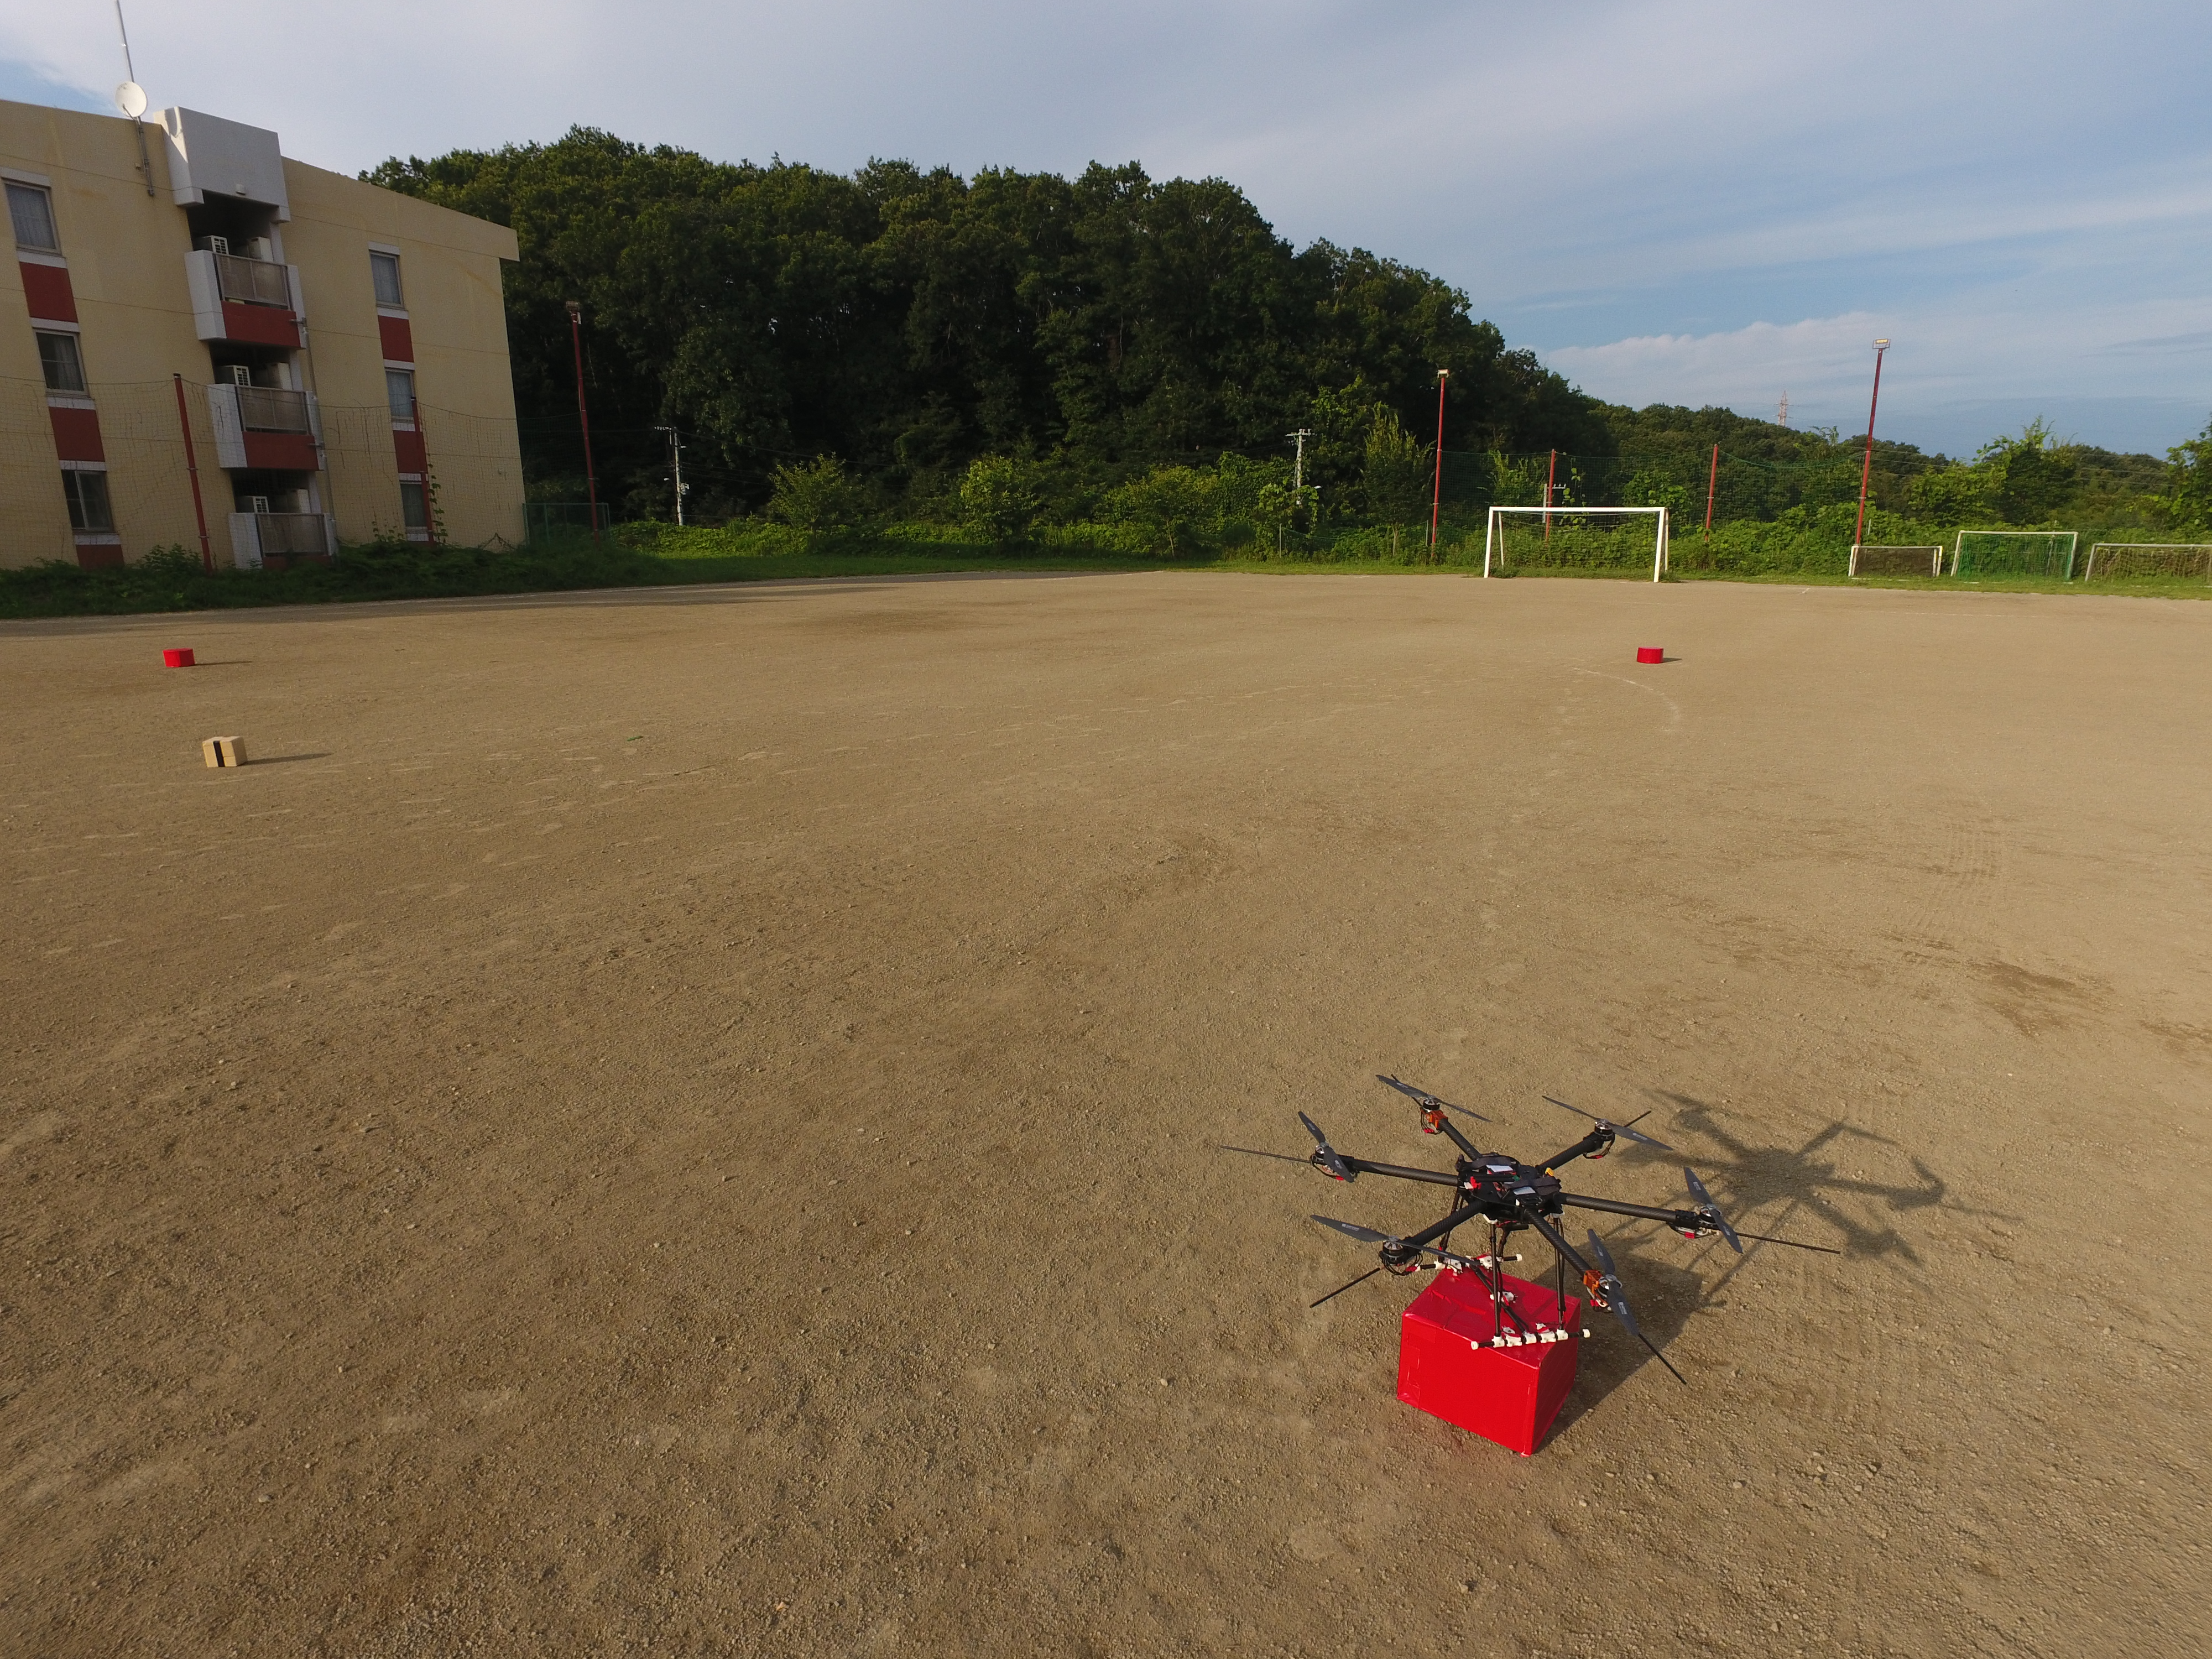
\includegraphics[width=\iwidth, height=\iheight]{sections/grand/images/DJI_0092}}\hspace{1.1em}%
   \caption{JSK--Team testbed setup at Hachioji, Tokyo, Japan}
   \label{fig:objects}
 \end{figure}


\end{document}


%\section{Future Plan}

\end{document}
